\documentclass{article}

% Marges du papier
\usepackage[a4paper, margin=3cm, top=2cm]{geometry}
\usepackage[utf8]{inputenc}
\usepackage[frenchb]{babel}

% Pas d'indentation de chaque début de paragraphe
\setlength{\parindent}{0pt}
\usepackage{listings}
\usepackage{color}
\usepackage[toc,page]{appendix}
\usepackage{booktabs}
\usepackage{csquotes}
\usepackage{adjustbox}
\usepackage{tcolorbox}
\usepackage{tabularx}
\usepackage{graphicx}
\usepackage{url}

% Pour que les footnotes dans les tableaux fonctionnent \begin{savenotes} <tableau> \end{savenotes}
\usepackage{footnote}

\usepackage{pdflscape}
\usepackage{fancyhdr}
\usepackage[style=verbose,backend=bibtex]{biblatex}

% Path du dossier dans lequel se trouvent les images
\graphicspath{ {img/} }

% numéro de citation entre crochets. Ex: [3]
\renewcommand*{\thefootnote}{[\arabic{footnote}]}

% "Annexes" en français au lieu de "Appencies"
\renewcommand{\appendixtocname}{Annexes}
\renewcommand{\appendixpagename}{Annexes} 


\definecolor{codegreen}{rgb}{0,0.6,0}
\definecolor{codegray}{rgb}{0.5,0.5,0.5}
\definecolor{codepurple}{rgb}{0.58,0,0.82}
\definecolor{backcolour}{rgb}{0.95,0.95,0.92}

% Crée une boîte "importante" \begin{important}Ceci est important\end{important}t
\newenvironment{important}
    {
		\begin{tcolorbox}
		\begin{center}
		\includegraphics[scale=0.3]{important}
		\end{center}
		\par
    }
	{
		\end{tcolorbox}
	}

\definecolor{tableheader}{rgb}{0.95,0.95,0.92}
 
\lstdefinestyle{mystyle}{
    backgroundcolor=\color{backcolour},   
    commentstyle=\color{codegreen},
    keywordstyle=\color{blue},
    numberstyle=\tiny\color{codegray},
    stringstyle=\color{codepurple},
    basicstyle=\footnotesize,
    breakatwhitespace=false,         
    breaklines=true,                 
    captionpos=b,                    
    keepspaces=true,                 
    numbers=left,                    
    numbersep=5pt,                  
    showspaces=false,                
    showstringspaces=false,
    showtabs=false,                  
    tabsize=2
}

\lstset{%
	inputencoding=utf8,
	extendedchars=true,
	literate=%
	{é}{{\'{e}}}1
	{è}{{\`{e}}}1
	{ê}{{\^{e}}}1
	{ë}{{\¨{e}}}1
	{É}{{\'{E}}}1
	{Ê}{{\^{E}}}1
	{û}{{\^{u}}}1
	{ù}{{\`{u}}}1
	{â}{{\^{a}}}1
	{à}{{\`{a}}}1
	{á}{{\'{a}}}1
	{ã}{{\~{a}}}1
	{Á}{{\'{A}}}1
	{Â}{{\^{A}}}1
	{Ã}{{\~{A}}}1
	{ç}{{\c{c}}}1
	{Ç}{{\c{C}}}1
	{õ}{{\~{o}}}1
	{ó}{{\'{o}}}1
	{ô}{{\^{o}}}1
	{Õ}{{\~{O}}}1
	{Ó}{{\'{O}}}1
	{Ô}{{\^{O}}}1
	{î}{{\^{i}}}1
	{Î}{{\^{I}}}1
	{í}{{\'{i}}}1
	{Í}{{\~{Í}}}1
}

\lstdefinestyle{json}
{
  showstringspaces    = false,
  keywords            = {false,true},
  alsoletter          = 0123456789.,
  morestring          = [s]{"}{"},
  basicstyle          = \ttfamily,
  keywordstyle        = \ttfamily\bfseries,
}
 
\lstset{style=mystyle}

\usepackage{fancyhdr}
 
\pagestyle{fancy}
\fancyhf{}
% Header left
\fancyhead[RE,LO]{
\includegraphics[width=4cm]{heiglogo}}

% Header height
\setlength\headheight{1.5cm}

% Header right
\fancyhead[LE,RO]{WEBRAILS - Julien Amacher, Romain Maillard}

% Footer right
\fancyfoot[LE,RO]{\thepage}

\usepackage{xcolor,colortbl}

\bibliography{biblio} 


\selectlanguage{french}

\title{Projet WEBRAILS}
\date{2016}
\author{Julien Amacher, Romain Maillard}

\begin{document}


% Page de garde
\makeatletter         
\def\@maketitle{
\raggedright

\includegraphics[width=6cm]{heiglogo}\\[8ex]
\begin{center}
{\Huge \bfseries \sffamily \@title }\\[4ex]
{\Large  \@author}\\[6ex]
\@date\\[20ex]

{\large News}\\[8ex] 

\end{center}}
\makeatother


\maketitle
\thispagestyle{empty}
\newpage
\thispagestyle{empty}
\tableofcontents
\newpage

\section{Introduction}

Ce projet a pour but de réaliser une plate-forme permettant d'une part la rédaction de news et d'autre part leur consultation. Les rédacteurs écrivent et modifient des news, en y liant des catégories (par ex: politique) et des sources (par ex: Paul Dupont). Chaque rédacteur travaille pour un média (par ex: France Info)

\section{Contraintes}

Les contraintes du projet sont les suivantes
\begin{itemize}
\item Le langage de programmation est Ruby on Rails (RoR)
\item La base de données est MySQL
\end{itemize}

\section{Cas d'utilisation}

Ce chapitre décrit les attentes et les fonctionnalités fournies pour chaque type de client de l’application.

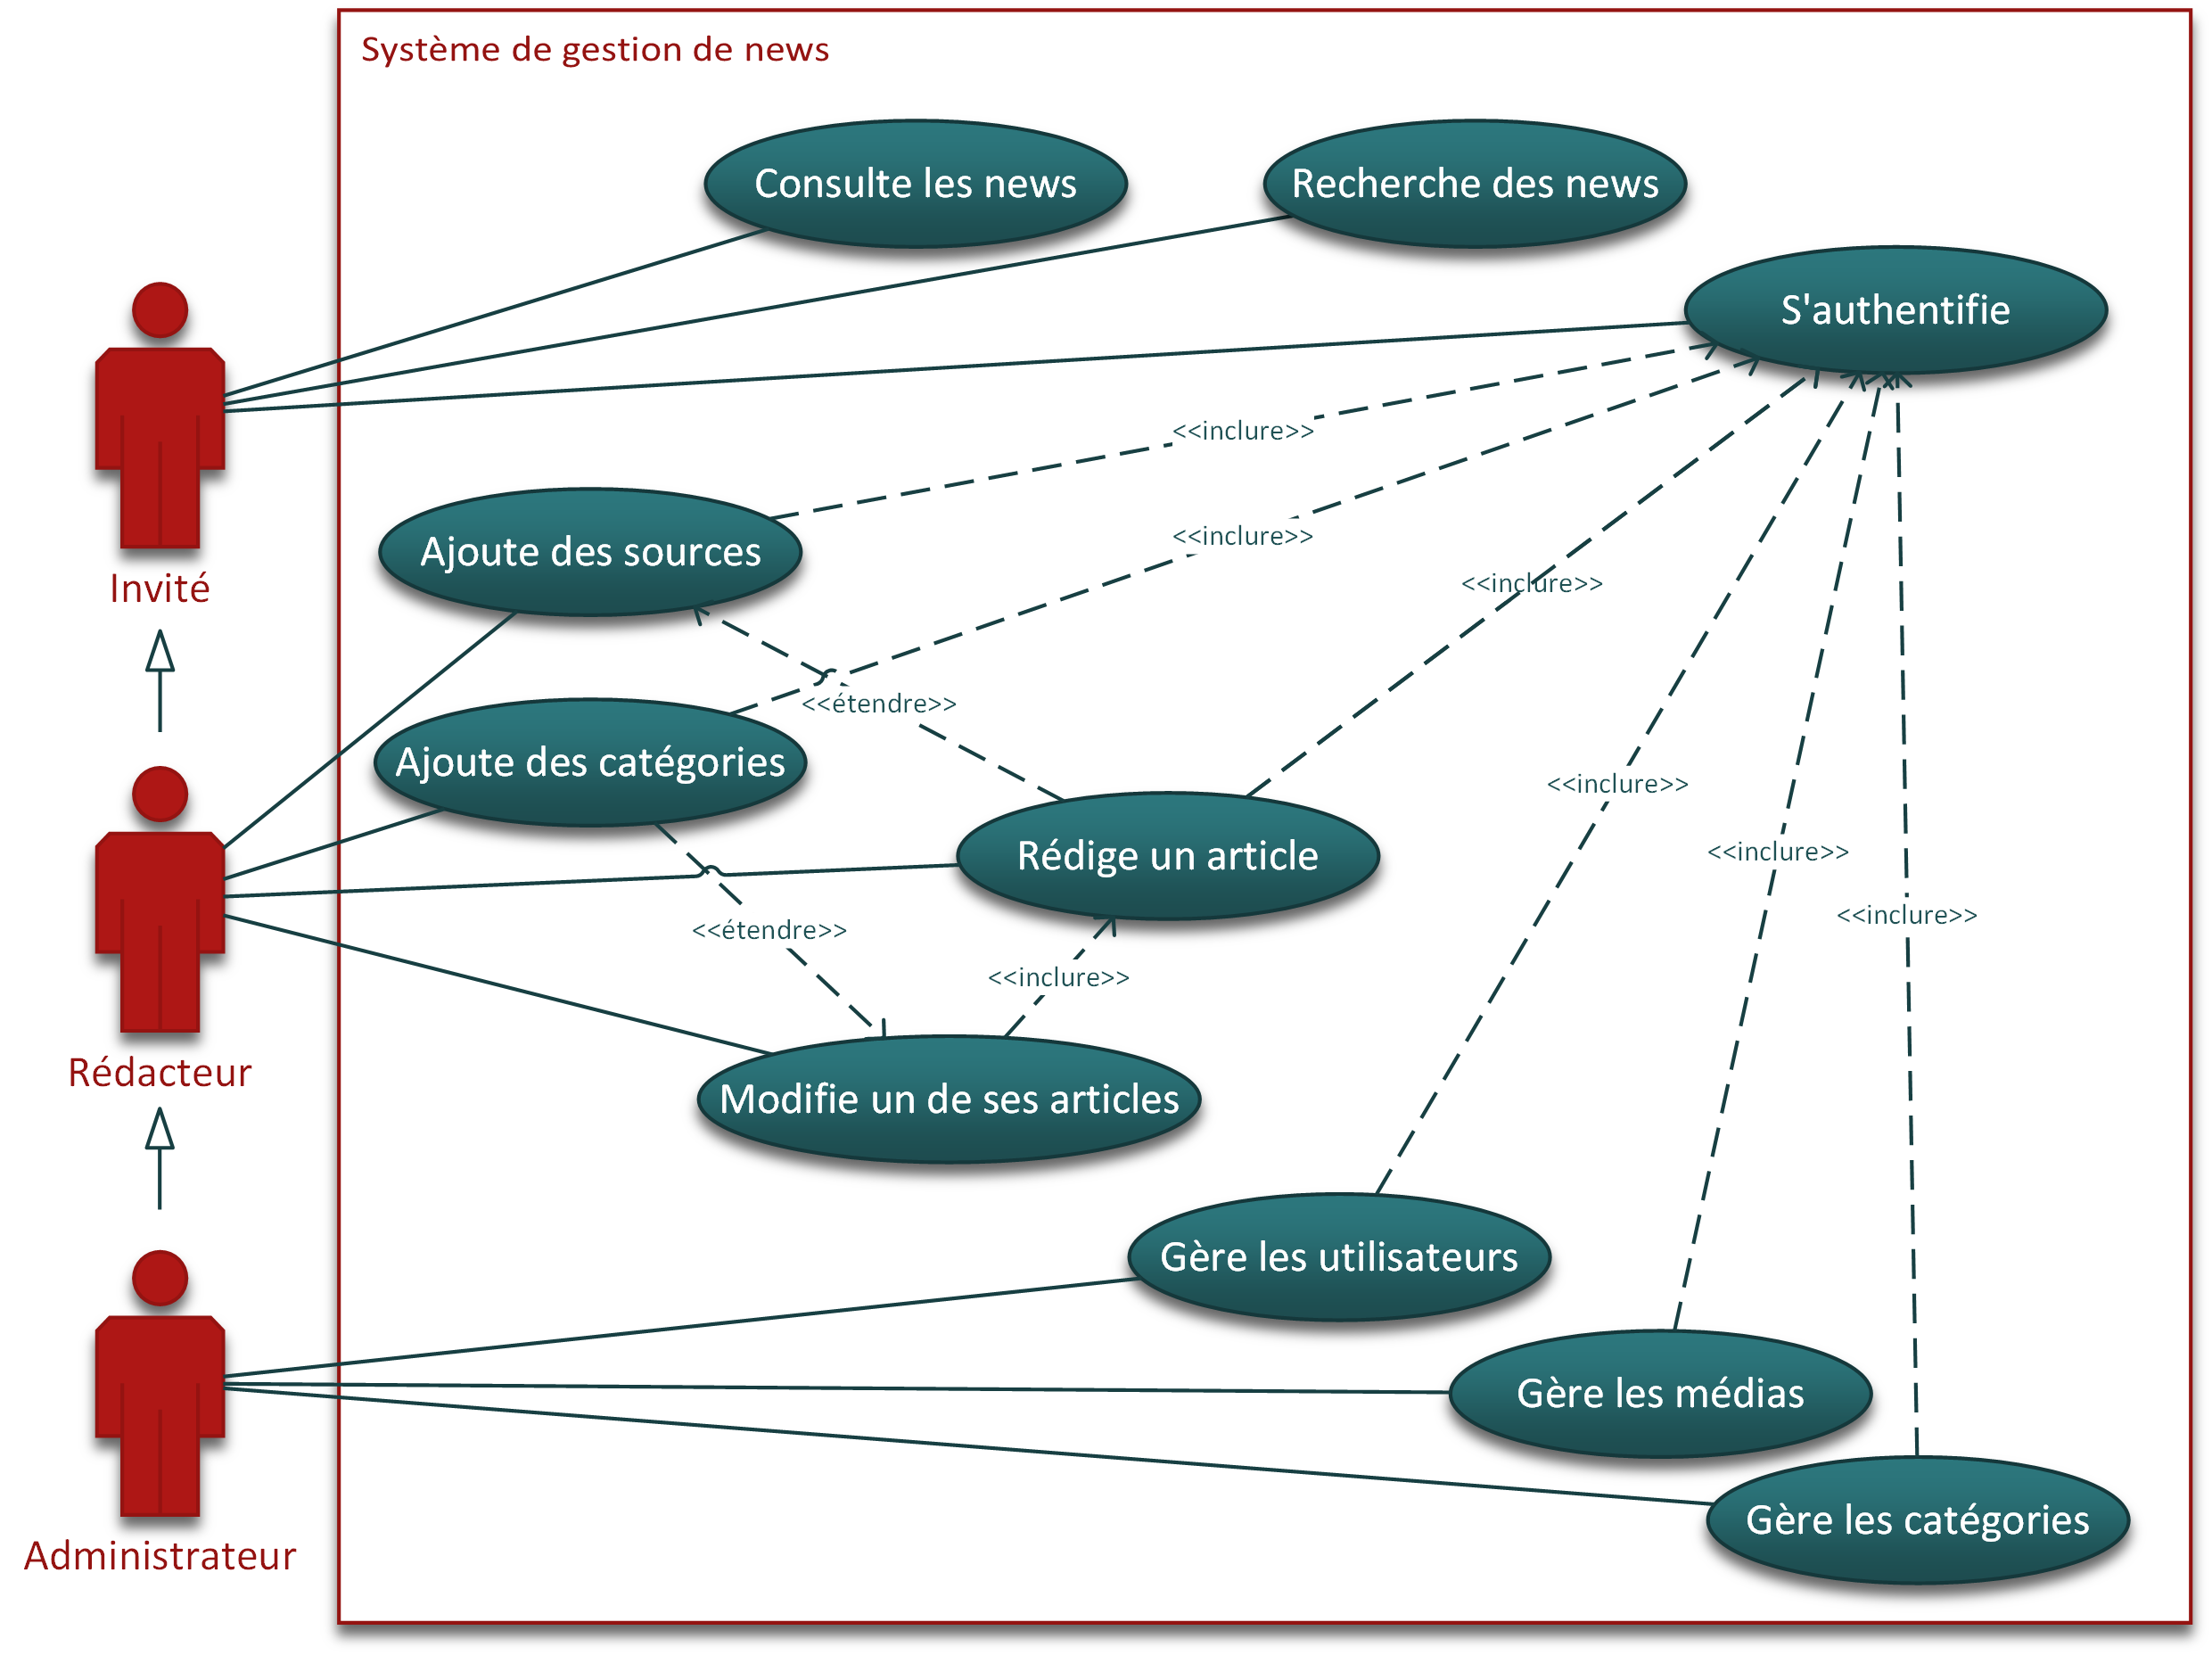
\includegraphics[width=\textwidth]{use_cases}


\subsection{Les invités}

\subsubsection{Consultent les news}

Ils peuvent librement consulter les news qu'ils désirent. Celles-ci sont présentes sur la page principale du site.

\subsubsection{S'authentifient}

Les invités s'authentifient en fournissant les informations suivantes :
\begin{itemize}
\item Leur adresse email
\item Leur mot de passe
\end{itemize}

Leur compte est ensuite identifié et leur rôle leur est attribué (rédacteur ou administrateur)

\subsubsection{Recherche des news}

Il est possible de rechercher une news par son titre, sa catégorie ou sa source.

\subsection{Les rédacteurs}

\subsubsection{Ajoutent une source à leur news}

Une news ayant au minimum une source, le rédacteur de la news peut en créer et en lier. Une news est consistuée d'un titre, d'un chapeau ainsi que d'un contenu. 

\subsubsection{Ajoutent une catégorie à leur news}

Une catégorie pouvant contenir plusieurs news (par exemple: politique), un rédacteur peut spécifier les catégories concernées par sa news.

\subsubsection{Rédigent une news}

Le rédacteur peut écrire une news. Une news comprend un titre, un chapeau (extrait en gras), un contenu ainsi qu'une liste de sources et est contenue dans au moins une catégorie.

Idéalement, les sources devraient pouvoir être créées `sur le vif` lors de la rédaction d'une news.

\subsubsection{Modifient une news}

Le rédacteur peut modifier une de ses news, cela inclut:
\begin{itemize}
\item Son titre
\item Son chapeau
\item Son contenu
\item Ses sources liées (en ajouter, en supprimer)
\item Ses catégories liées (en ajouter, en supprimer)
\end{itemize}

\subsection{Un administrateur}

\subsubsection{Gère les utilisateurs}

Un administrateur crée, modifie et supprime les comptes des utilisateurs du système.

\subsubsection{Gère les catégories}

Un administrateur gère les catégories : il peut en ajouter, en modifier et en supprimer.

\subsubsection{Gère les médias}

Un administrateur gère les médias : il peut en ajouter, en modifier et en supprimer. Chaque rédacteur est lié à un média et l'administrateur est le seul à pouvoir modifier le média au quel le rédacteur est rattaché.

\newpage
\section{Base de données}

\subsubsection{MCD}

Le modèle conceptuel des données se présente comme suit:

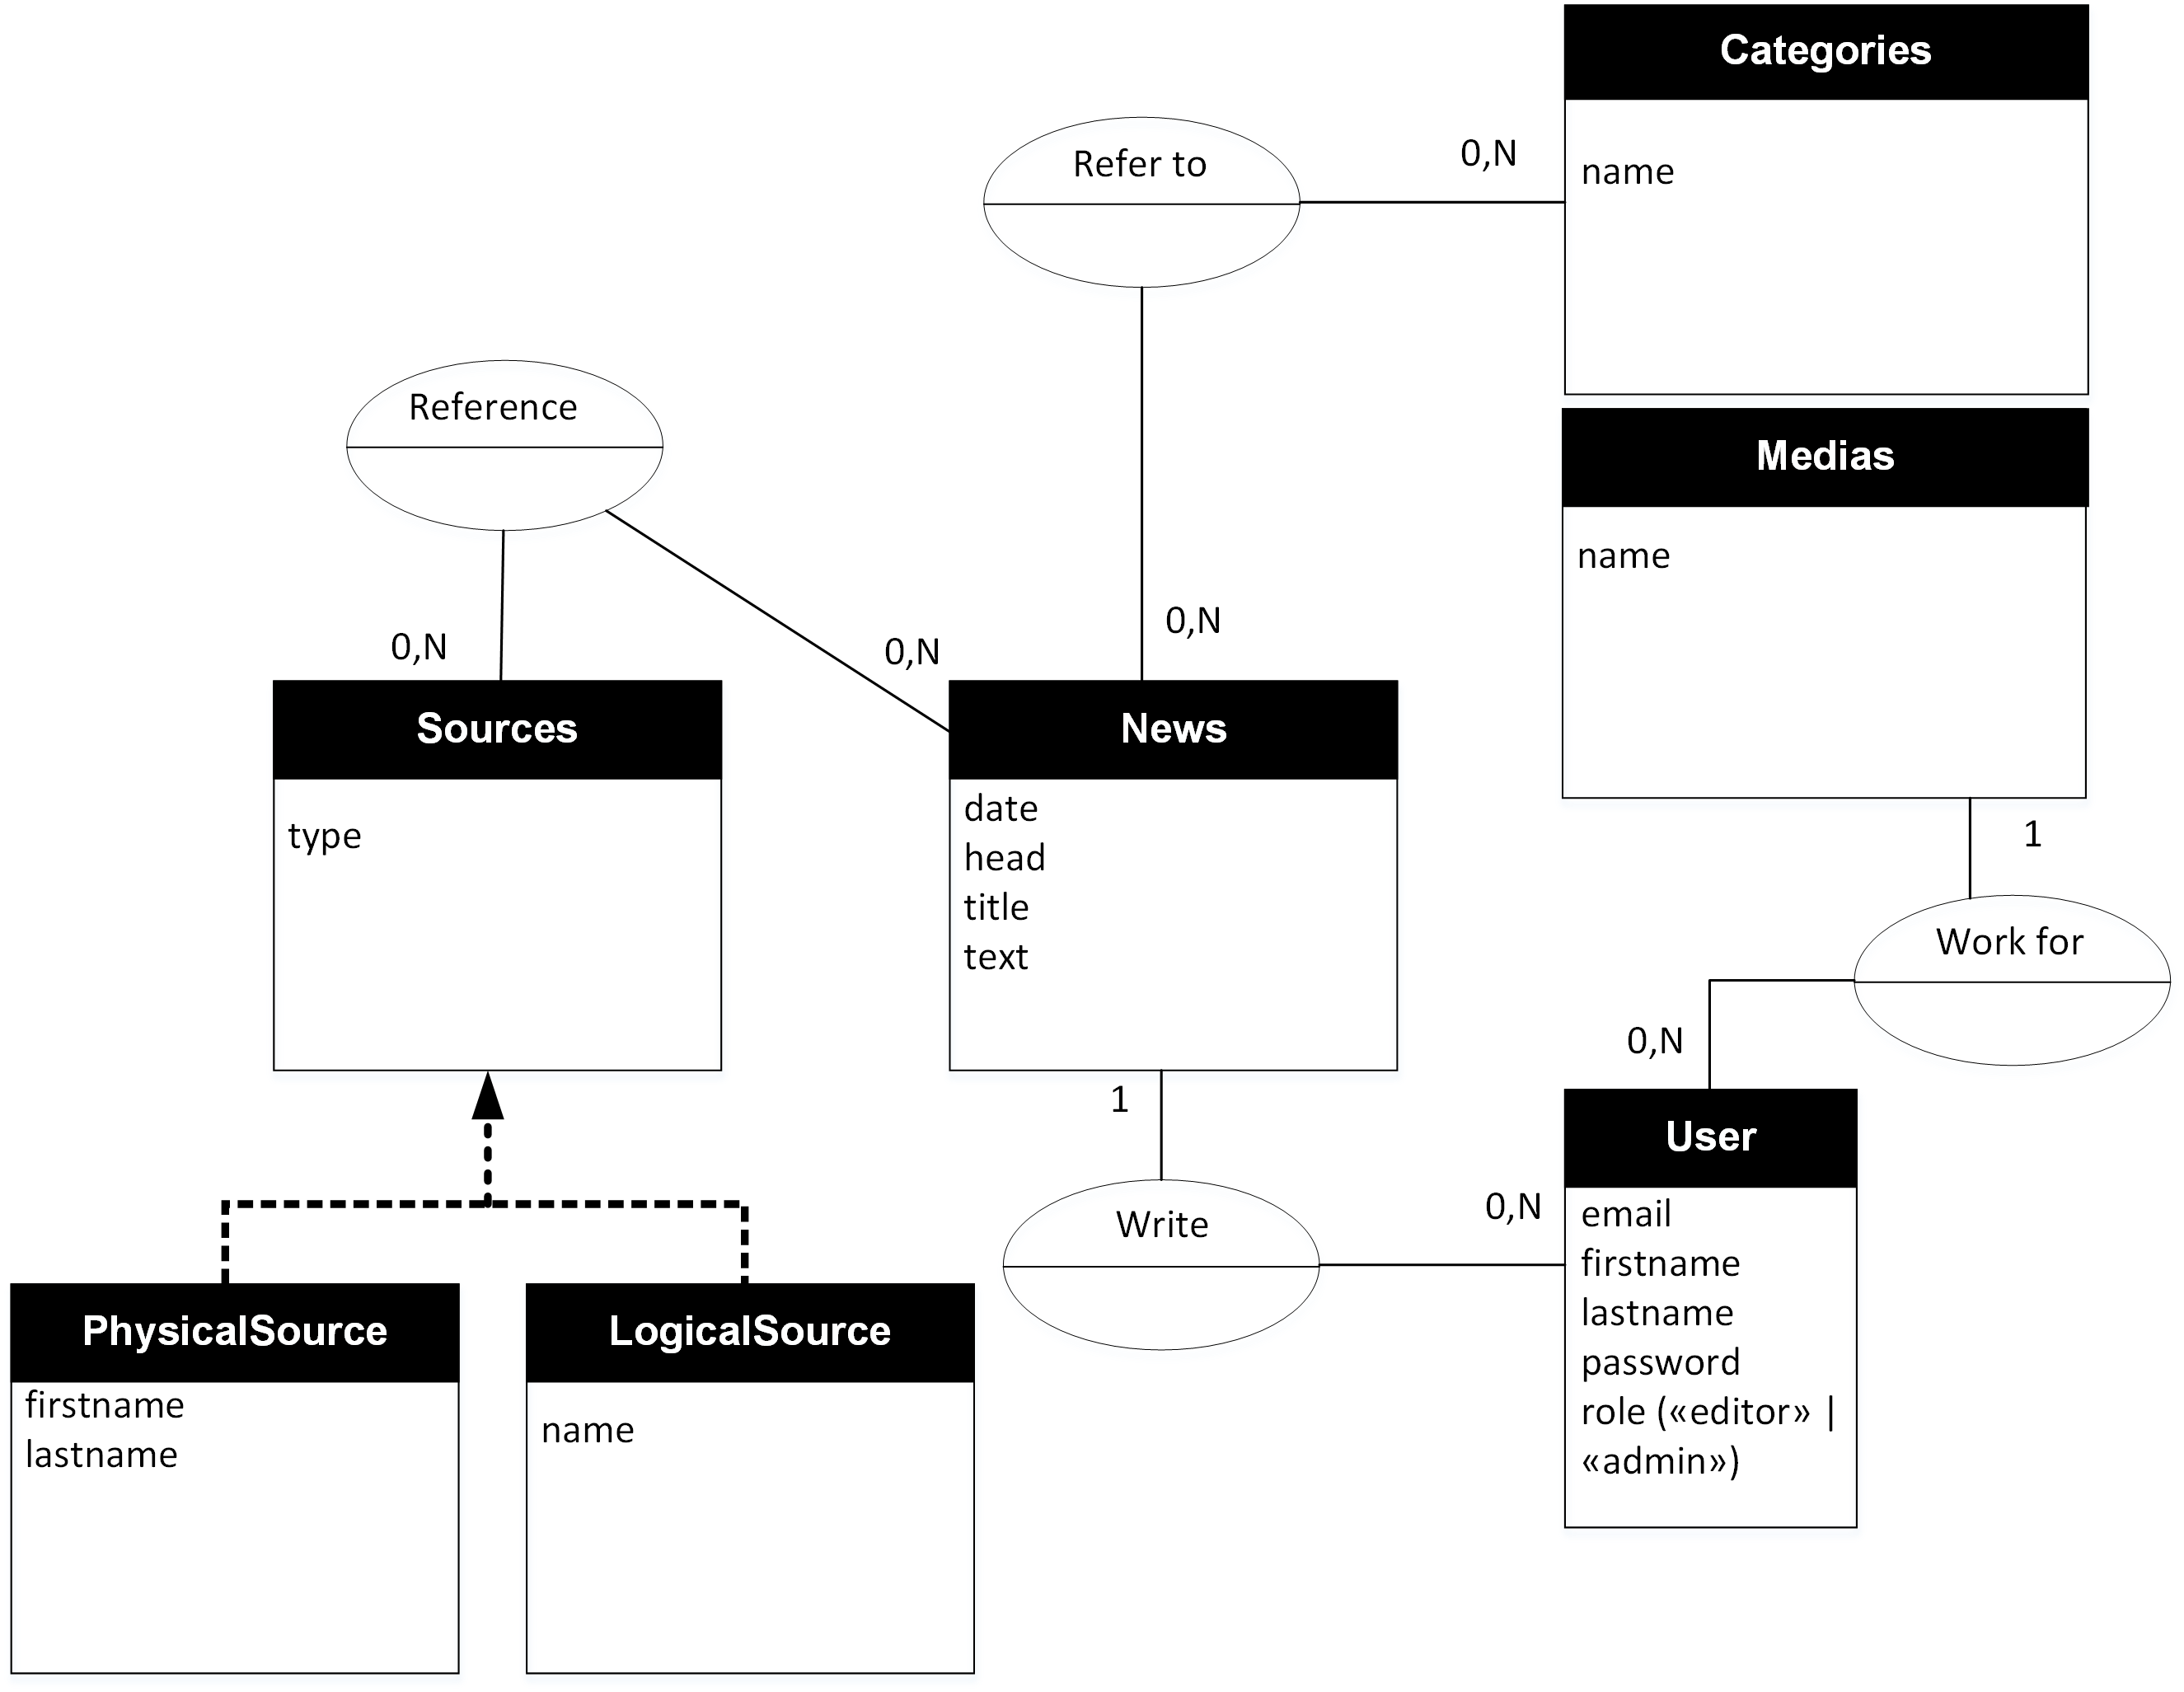
\includegraphics[width=\textwidth]{mcd}

Contraintes:
\begin{itemize}
\item Une news a au minimum une source liée
\item Une source fait référence à au minimum une catégorie (politique, économie, etc.)
\item Une source peut exister même si aucune news n'y fait référence, idem pour les catégories de news
\item Un rédacteur est lié à un média
\end{itemize}

\subsubsection{MPD}

\textbf{Users}

\begin{itemize}
\item firstname
\item lastname
\end{itemize}

Cancancan gère le rôle de l'utilisateur et Devise gère l'authentification (et y ajoute l'attribut email).

\textbf{Report}

\begin{itemize}
\item head
\item title
\item text
\end{itemize}

Chaque rapport a une date de création. Nous utilisons le champ created at de Rails.

\textbf{Sources}

\begin{itemize}
\item firstname
\item lastname
\item name
\item type
\end{itemize}

\textbf{Categories}

\begin{itemize}
\item name
\end{itemize}

\textbf{Medias}

\begin{itemize}
\item name
\end{itemize}

\section{Itérations}

\begin{itemize}
\item 3 mai
	\begin{itemize}
	\item Création de la base de données et des pages squelettes.
	\end{itemize}
	
\item 17 mai
	\begin{itemize}
	\item Ajout, modification et suppression de news, utilisateurs, catégories et médias fonctionnent.
	\end{itemize}

\item 7 juin
	\begin{itemize}
	\item Fonctionnalité de recherche terminée + droits d'accès implémentés.
	\end{itemize}
\end{itemize}

\section{Fonctionnalités Ajax}

La recherche des news se fait via Ajax. La recherche se fait par news, catégorie et source. Le contenu, titre et chapeau de la news sont considérés lors de la recherche.

\section{Manuel utilisateur}

Disponible en annexe.

\section{Configuration CanCanCan}

La restriction de l'exécution en fonction des rôles est implémentée comme suit dans le fichier ability.rb:
\begin{lstlisting}
class Ability
  include CanCan::Ability

  def initialize(user)
    user ||= User.new
	
	if user.role == "admin"
		can :manage, :all
		can :reset_password, User
	end
	
	if user.role == "author"
		can :manage, Report
		can :manage, Source
	end
	
	can :read, Report
	can :read, Category
	can :read, Source
  end
end
\end{lstlisting}

\section{Implémentation Ajax}

Notre fonctionnalité de recherche a été implémentée en utilisant les mécanismes de requête HTTP accessibles depuis Javascript (Ajax)

Le but est le suivant: lorsqu'un terme de recherche est entré, une recherche est effectuée dans le but de trouver les news, catégories, sources et médias correspondants.
A cet effet, la recherche s'opère:
\begin{itemize}
\item Le titre des news
\item Le chapeau des news
\item Le contenu des news
\item Le nom des catégories
\item Le nom des sources (s'il s'agit d'une source de type "entité morale") ainsi que le prénom/nom s'il s'agit d'une source de type "personne physique"
\item Le nom des sources
\item Le nom des médias
\end{itemize}

Ces résultats sont ensuite présentés à l'utilisateur, les entrées sont cliquables:

\begin{figure}[h]
  \centering
  
\includegraphics[width=10cm]{recherche_ajax}
\end{figure}

Le champ texte d'entrée présenté à l'utilisateur est surveillé et toute modification y relative entraîne l'appel de la fonction suivante:

\begin{lstlisting}
$(function() {
	$('#search_terms').on('input', function() {
		var search_terms = $(this).val();
		
		if (search_terms == "") {
			$('#search_div').html("");
		} else {
			$.get("/reports/search", {"search_terms": search_terms }, function(data) {
				$('#search_div').html(data);
			});
		}
	});
});
\end{lstlisting}

Le contrôleur "report" (méthode "search") se charge d'effectuer cette recherche:

\begin{lstlisting}
def search
	@search_terms = params[:search_terms]
	@search_results = Hash.new
	@search_results["reports"] = Report.where("title LIKE ? OR head LIKE ? OR text LIKE ?", "%#{@search_terms}%", "%#{@search_terms}%", "%#{@search_terms}%").order("updated_at DESC").limit(20)
	@search_results["categories"] = Category.where("name LIKE ?", "%#{@search_terms}%")
	@search_results["sources"] = Source.where("firstname LIKE ? OR lastname LIKE ? OR name LIKE ?", "%#{@search_terms}%", "%#{@search_terms}%", "%#{@search_terms}%")
	@search_results["medias"] = Medium.where("name LIKE ?", "%#{@search_terms}%")
	
	render :partial => "reports_search"
end
\end{lstlisting}

\newpage
\section{Déploiement}

La procédure suivante permet de déployer l'application et de la tester. Nous utilisons les fixtures pour permettre de charger directement la base de données avec des données de test.

\begin{itemize}
\item Créer la base de données nommée "news"
\item Exécuter: \begin{verbatim}bundle install\end{verbatim}
\item Exécuter: \begin{verbatim}rake db:migrate\end{verbatim}
\item Exécuter: \begin{verbatim}rake db:fixtures:load\end{verbatim}
\item Exécuter: \begin{verbatim}rails s\end{verbatim}
\end{itemize}

\par\null\par

Les comptes créés par les fixtures sont les suivants (email password):

\begin{itemize}
\item admin: jean@paul.com \begin{verbatim}tn^VQBaw\end{verbatim}
\item auteur: albert@haller.com \begin{verbatim}48n6dqBe\end{verbatim}
\item auteur: jaime@heig.com \begin{verbatim}gJWOp74\end{verbatim}
\end{itemize}

\newpage
\section{MVC}

Le mécanisme MVC utilisé est celui fourni par Ruby on Rails.

\par\null\par

Les contrôleurs implémentés sont les suivants:

\begin{figure}[h]
  \centering
  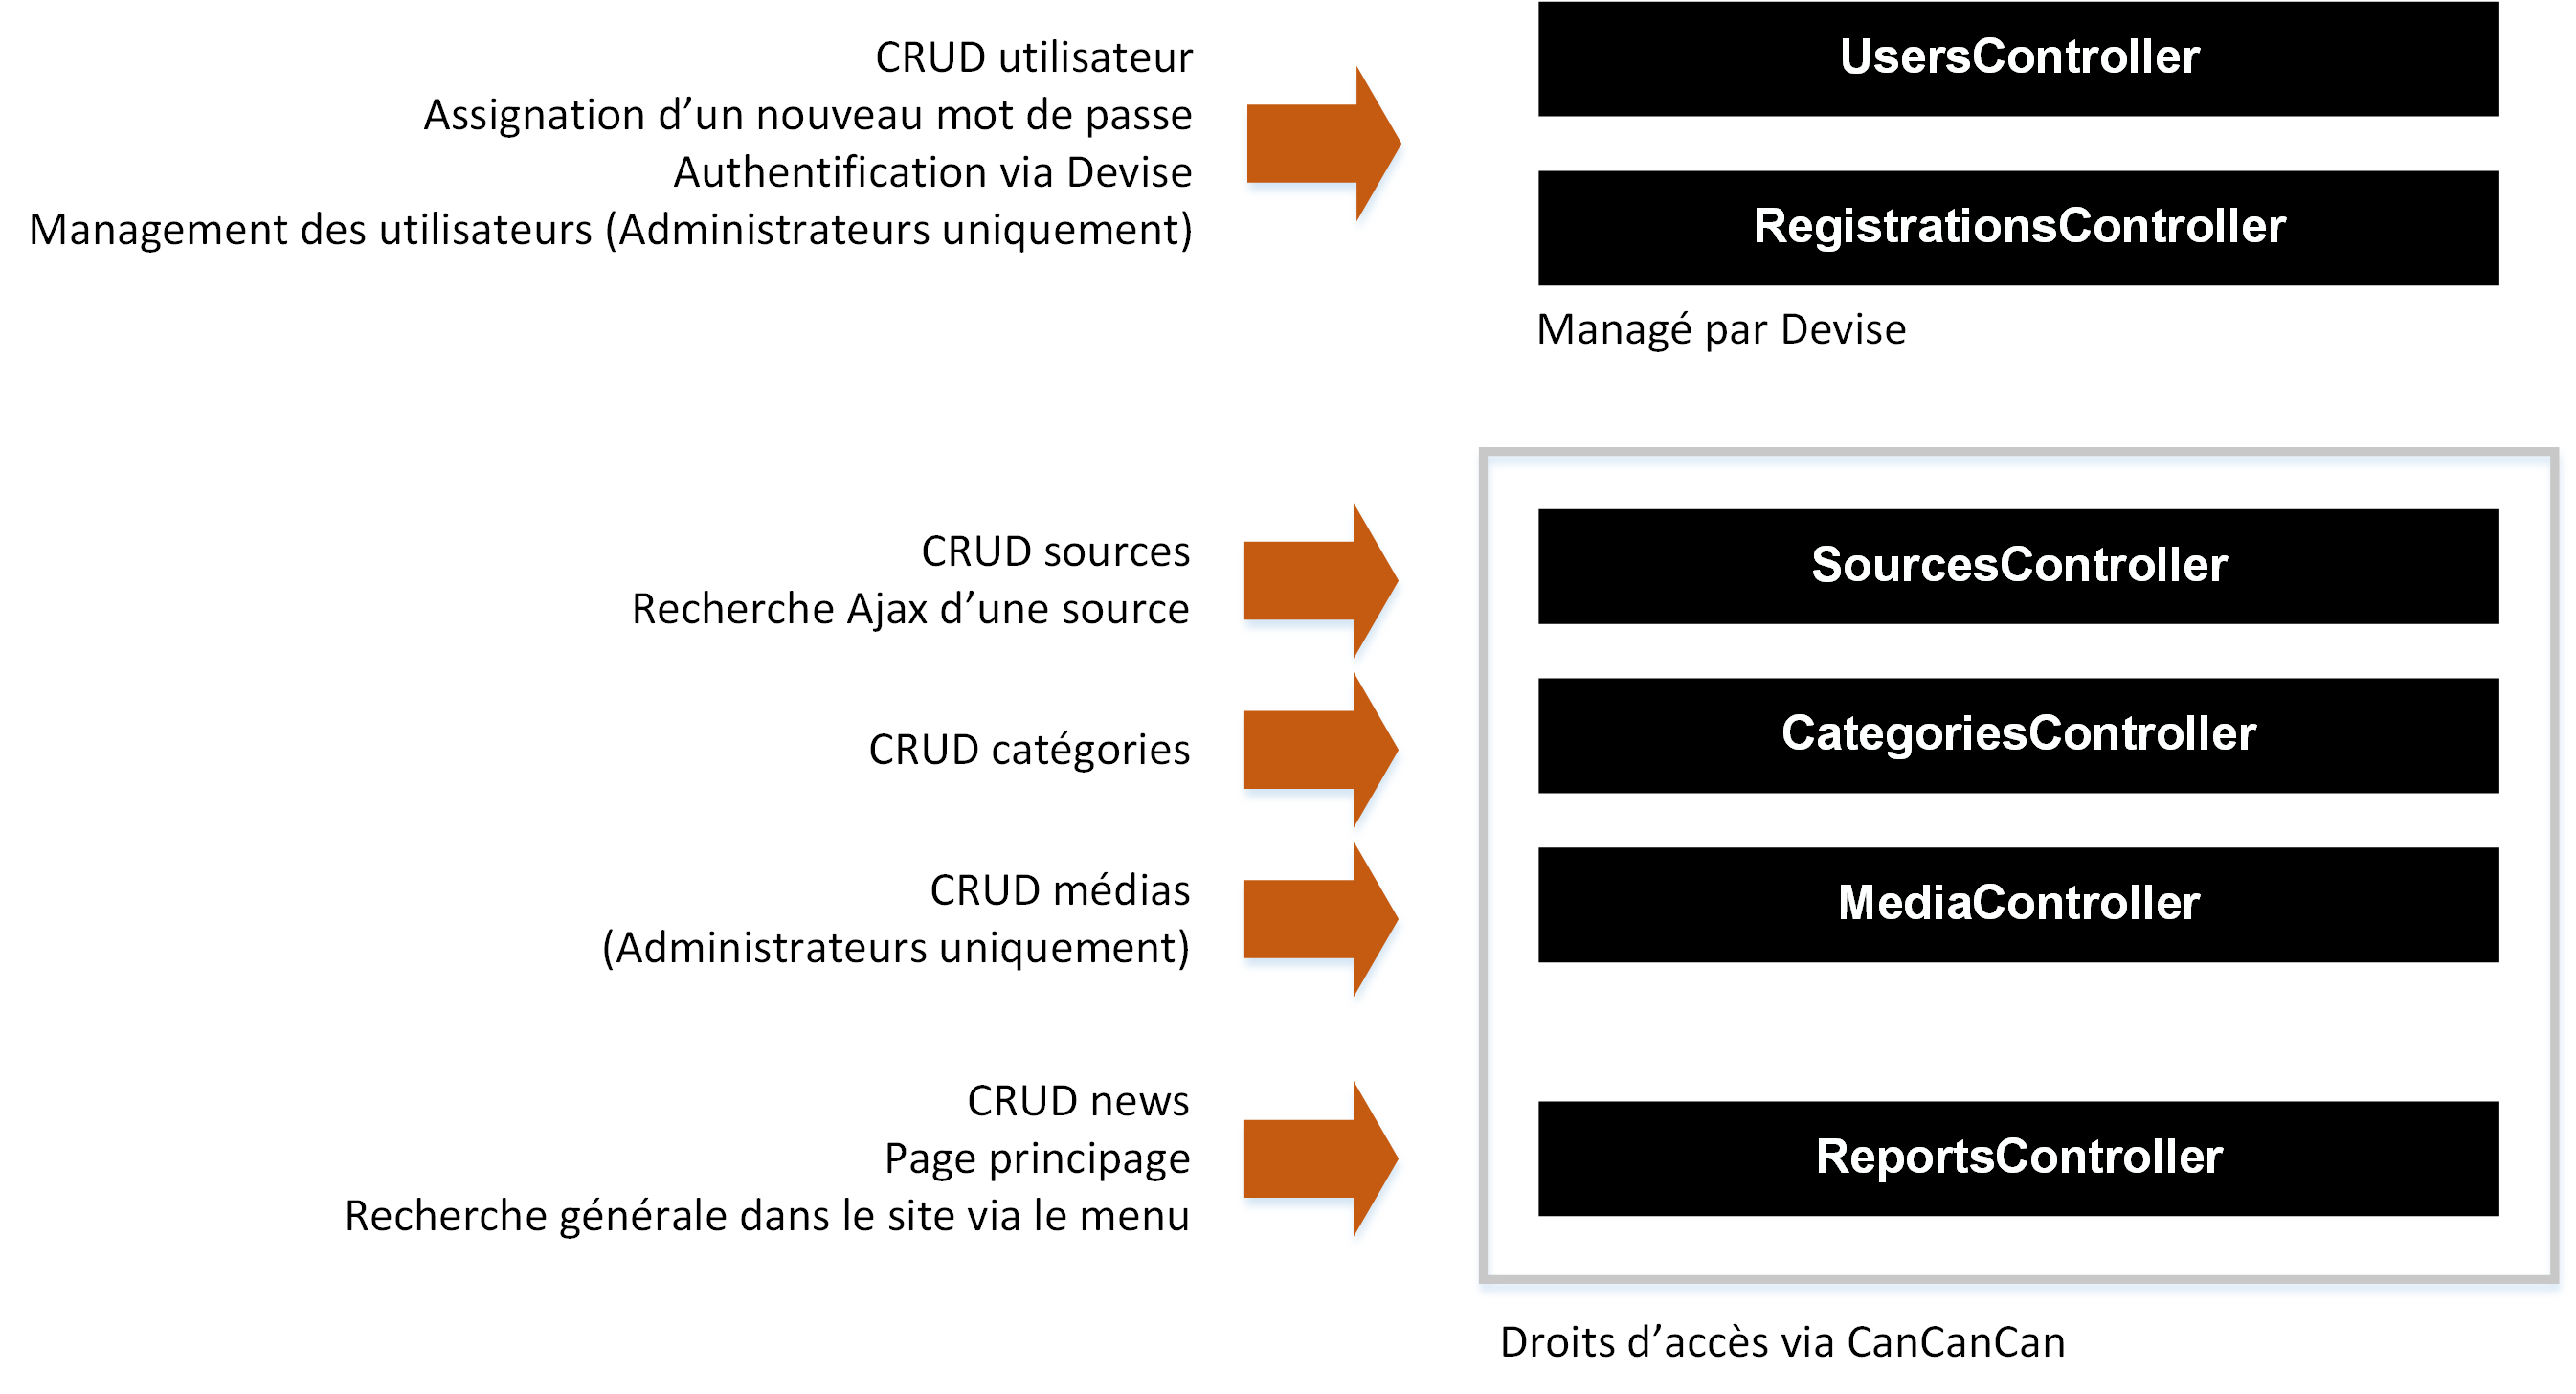
\includegraphics[width=14cm]{mvc}
\end{figure}

Les relations ORM propres à Rails implémentées sont les suivantes:

\begin{figure}[h]
  \centering
  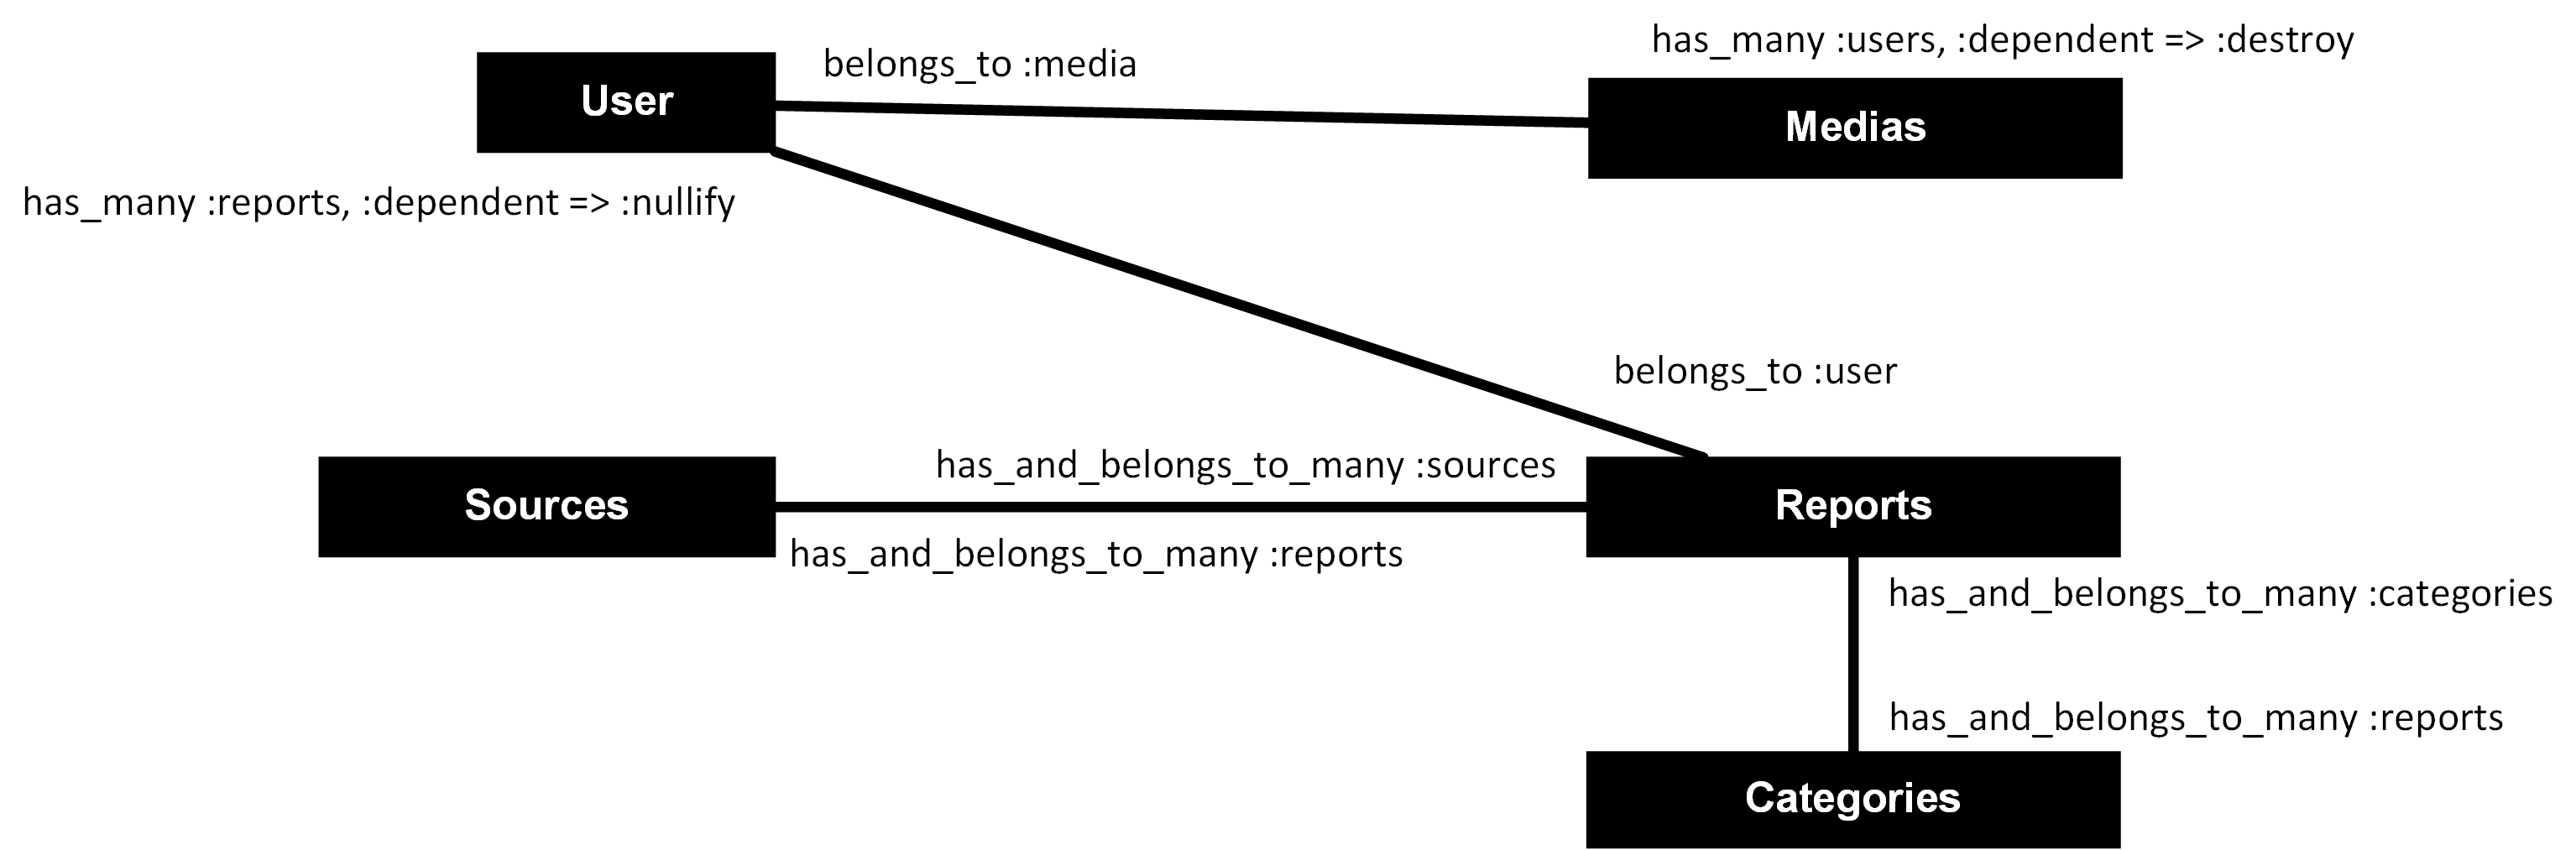
\includegraphics[width=14cm]{relations}
\end{figure}

\section{Librairies utilisées}

Les librairies suivantes ont été réalisées:

\begin{itemize}
\item Bootstrap, pour les styles graphiques
\item Devise, pour l'authentification
\item CanCanCan, pour la gestion des droits d'accès
\end{itemize}

\par\null\par

Turbolinks a été désactivé, car le Javascript n'était pas correctement exécuté lorsque la page était chargée et il fallait rafraîchir la page pour que le Javascript soit enfin chargé.

\section{Etat des lieux}

Le projet est fonctionnel et utilisable. Il répond au cahier des charges.

\newpage
\section{Conclusion}

Ce projet a été une bonne prise en main de RoR. Nous avons pu consulter ses forces mais également ses faiblesses. Ruby est agréable à utiliser car il permet la génération rapide de squelettes, mais cet avantage a ses limites et un inconvénient majeur est de devoir revoir chaque interface pour y ajouter les relations manquantes. Au niveau organisation, il n'a pas toujours été facile de trouver le temps de travailler sur le projet, compte tenu de notre charge de travail tout au long de ce semestre. En bref, ce projet a été fort utile pour appuyer et mettre en oeuvre ce que nous avons appris durant le cours.

\printbibliography

\newpage
\begin{appendices}

\newpage
\section{Manuel utilisateur}
%\newpage
%\section{Annexe 2}
\end{appendices}

\end{document}